\newcommand{\timeconv}[2]{\ensuremath{\mathtt{Conv}_{#1}(#2)}}
\newcommand{\applyBlocks}[2]{\ensuremath{\mathtt{apply}_\mathit{#1}(#2)}}
\newcommand{\ledgertip}[1]{\ensuremath{\mathtt{tip}(#1)}}
\newcommand{\switch}[3]{\ensuremath{\mathtt{switch}_{(\mathit{#1},\;\mathit{#2})}(#3)}}

\chapter{Time}
\label{time}

\section{Introduction}
\label{time:introduction}

A fundamental property of the Ouroboros family of consensus protocols is that
they all divide time into discrete chunks called \emph{slots}; typically the
duration of a slot is on the order of seconds. In most Ouroboros protocols slots
are grouped into \emph{epochs}, with certain changes to the consensus chain
state happening at various points in an epoch. All nodes running the blockchain
agree on a \emph{system start time} (as a UTC time) through the chain's genesis
configuration, making the translation from a particular wallclock time to a slot
number easy: subtract the system start time from the wall clock time, and
divide by the slot length. This assumption that the mapping between wall clock
and slot or epoch numbers is always available permeated the consensus layer.
Unfortunately, it is not a valid assumption in the presence of hard forks.

It's not difficult to illustrate this with an example. Suppose we want to know
which slot time $t$ corresponds to in:
%
\begin{center}
\begin{tikzpicture}
\draw (0,0) -- (330pt, 0);
\draw [dotted] (180pt,20pt) node[above] {era transition} -- (180pt,-30pt);
\node at (273 pt,0) {$\bullet$};
\node at (273 pt,0) [above] {$t$};
% era 1
% slot length 6
% epoch size 10
% 3 epochs
\foreach \x in {0, 6, ..., 180} {
  \draw (\x pt, 0) -- +(0, -3pt);
}
\foreach \x in {0, 60, ..., 180} {
  \draw (\x pt, 0) -- +(0, -10pt);
}
% era 2
% slot length 3
% epoch size 16
% 3+ epochs
\foreach \x in {180, 183, ..., 330} {
  \draw (\x pt, 0) -- +(0, -3pt);
}
\foreach \x in {180, 228, ..., 330} {
  \draw (\x pt, 0) -- +(0, -10pt);
}
\end{tikzpicture}
\end{center}
%
We can read off from this depiction that $t$ is in epoch 1 \emph{of the second
era}, and relative slot 14 within that epoch. Since there are 16 slots to an
epoch in that era, that makes it slot $1 \times 16 + 14 = 30$ within that era.
The second era was preceded by three epochs in the first era, each of which
contained 10 slots, which means that time $t$ was slot $3 \times 10 + 30 = 60$
globally.

But now consider how this calculation changes if the era transition would have
happened one epoch later:
%
\begin{center}
\begin{tikzpicture}
\draw (0,0) -- (330pt, 0);
\draw [dotted] (240pt,20pt) node[above] {era transition} -- (240pt,-30pt);
\node at (273 pt,0) {$\bullet$};
\node at (273 pt,0) [above] {$t$};
% era 1
% slot length 6
% epoch size 10
% 4 epochs
\foreach \x in {0, 6, ..., 240} {
  \draw (\x pt, 0) -- +(0, -3pt);
}
\foreach \x in {0, 60, ..., 240} {
  \draw (\x pt, 0) -- +(0, -10pt);
}
% era 2
% slot length 3
% epoch size 16
% 1+ epochs
\foreach \x in {240, 243, ..., 330} {
  \draw (\x pt, 0) -- +(0, -3pt);
}
\foreach \x in {240, 288, ..., 330} {
  \draw (\x pt, 0) -- +(0, -10pt);
}
\node at (273 pt,0) {$\bullet$};
\node at (273 pt,0) [above] {$t$};
\end{tikzpicture}
\end{center}
%
Slot $t$ is now in epoch 0 of the second era, with relative
slot 11, making it slot $0 \times 16 + 11 = 11$ within the second era.
Since the second era got preceded by \emph{four} epochs of the first era,
that makes time $t$ global slot $4 \times 10 + 11 = 51$.

All of this would be no more than a minor complication if the exact moment of
the era transition would be statically known. This however is not the case: the
moment of the era transition is decided \emph{on the chain itself}. This leads
to the inevitable conclusion that time/slot conversions depend on the ledger
state, and may indeed be impossible: the slot at time $t$ is \emph{simply not
yet known} if the transition to era 2 has not been decided yet.

\section{Slots, blocks and stability}
\label{time:slots-vs-blocks}

In \cref{consensus:overview:k} we discussed the fundamental parameter $k$:
blocks that are more than $k$ blocks away from the tip of the chain are
considered to be immutable by the consensus layer and no longer subject to
rollback. We say that such blocks are \emph{stable}.

The ledger layer itself also depends on stability; for example, in Shelley the
stake distribution to be used for the leadership check needs to be stable before
it is adopted (this avoids malicious nodes from inspecting the leadership
schedule and then trying to cause a rollback if that leadership schedule is not
beneficial to them).

The ledger layer however does not use block numbers to determine stability, but
uses slot numbers to approximate it instead. This ultimately comes from the fact
that in Ouroboros the length of an \emph{epoch} is based on slots, not blocks,
although this is something we may wish to revisit (\cref{future:block-vs-slot}).

Depending on the particular choice of consensus algorithm, not all slots contain
blocks. For example, in Praos only a relatively small percentage of slots
contain blocks, depending on the Praos $f$ parameter (in Shelley, $f$ is set to
5\%). However,  the various Ouroboros protocols come with proofs (actually, a
probabilistic argument) providing a window of a certain number of slots that is
guaranteed to contain at least $k$ blocks; for example, for Ouroboros Classic
that window is $2k$ slots\footnote{Without much justification, we adopt this
same window for PBFT as well. It is almost certainly a gross overestimation.},
and for Ouroboros Praos that window is $3k/f$. Stability requirements in the
ledger then take the form ``at least $3k/f$ slots must have passed'' instead of
``at least $k$ blocks must have been applied''.

\section{Definitions}

\subsection{Time conversion}

As we saw in \cref{time:introduction}, we cannot do time conversions independent
of a ledger state. This motivates the following definition:

\begin{definition}[Time conversion]
Let $\timeconv{\sigma}{t}$ be the function that converts time $t$, with $t$
either specified as a wallclock time, a slot number, or an epoch number, to a
triplet
\begin{center}
(wallclock time, slot number, epoch number)
\end{center}
using ledger state $\sigma$, provided $\sigma$ contains sufficient information
to do so; $\timeconv{\sigma}{t}$ is undefined otherwise.
\end{definition}

Since all past era transitions are (obviously) known, time conversion should
always be possible for points in the past. Let $\ledgertip{\sigma}$ be the (time
of) the most recently applied block in $\sigma$. Then:

\begin{property}[Conversion for past points]
$\timeconv{\sigma}{t}$ should be defined for all $t \le \ledgertip{\sigma}$.
\end{property}

Furthermore, we assume that time conversion is monotone:

\begin{property}[Monotonicity of time conversion]
\label{time-conversion-monotone}
If $\timeconv{\sigma}{t}$ is defined, then $\timeconv{\applyBlocks{bs}{\sigma}}{t}$ must be as well and
\begin{equation*}
\timeconv{\applyBlocks{bs}{\sigma}}{t} = \timeconv{\sigma}{t}
\end{equation*}
\end{property}
%
where $\applyBlocks{bs}{\sigma}$ denotes the ledger state after applying blocks
$\mathit{bs}$.

\subsection{Forecast range}

Under certain conditions a ledger state may be usable to do time conversions
for slots ahead of the ledger state.

\begin{definition}[Forecast range]
We say that time $t > \ledgertip{\sigma}$ is within the forecast range of
$\sigma$ if \timeconv{\sigma}{t} is defined.
\end{definition}

Note that monotonicity (\cref{time-conversion-monotone}) should still
apply.

\subsection{Safe zone}

In order to be able to have a non-empty forecast range, we need to restrict
when era transitions can occur.

\begin{definition}[Safe zone]
A \emph{safe zone} is a period of time ahead of a ledger's tip in which an
era transition is guaranteed not to occur if it is not yet known.
\end{definition}

Intuitively, a non-empty safe zone means that there will be time between an
era transition being announced and it happening, no matter how the chain
is extended (no matter which blocks are applied):
%
\begin{equation}
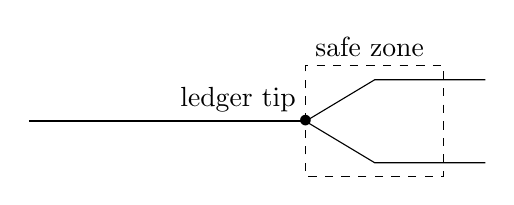
\begin{tikzpicture}[baseline=0pt]
\draw [thick] (-50pt,0) -- (50pt, 0) coordinate (tip);
\draw (tip) -- ++(25pt,  15pt) -- ++(40pt, 0pt);
\draw (tip) -- ++(25pt, -15pt) -- ++(40pt, 0pt);
\node at (tip) {$\bullet$};
\node at (tip) [above left] {ledger tip};
\draw [dashed] (tip)
            -- ++(0pt, 20pt) node[above right] {safe zone}
            -- ++(50pt, 0pt) -- ++(0pt, -40pt) -- ++(-50pt, 0pt) -- cycle;
\end{tikzpicture}
\end{equation}

\section{Ledger restrictions}
\label{time:ledgerrestrictions}

\subsection{Era transitions must be stable}

Monotonicity (\cref{time-conversion-monotone}) only talks about a chain's linear
history; since the consensus layer needs to deal with rollbacks (switching to
alternative chains) too, we will actually need a stronger property. Clearly,
time conversions cannot be invariant under switching to arbitrary chains; after
all, alternative chains might have era transitions in different places. The
consensus layer however does not \emph{support} switching to arbitrary
alternative chains; we have a maximum rollback (\cref{consensus:overview:k}),
and we never switch to a shorter chain (\cref{consensus:overview:chainsel},
\cref{never-shrink}). This means that we can model switching to an alternative
chain as $$\switch{n}{bs}{\sigma}$$ where $n \le k$ indicates how many blocks we
want to rollback, $\mathit{bs}$ is a list of new blocks we want to apply, and
$\mathtt{length} \; \mathit{bs} \ge n$.

\begin{property}[Time conversions stable under chain evolution]
\label{time-stable-under-evolution}
If \timeconv{\sigma}{t} is defined, then so is
\timeconv{\switch{n}{bs}{\sigma}}{t}
and moreover
\begin{equation*}
  \timeconv{\sigma}{t}
= \timeconv{\switch{n}{bs}{\sigma}}{t}
\end{equation*}
\end{property}

Intuitively, \cref{time-stable-under-evolution} says that we might not be able
to do time conversion for some time $t$ because it's outside our current forecast
range, but \emph{if} it is within forecast range, then we don't need to earmark
the answers we get from conversion as ``subject to rollback'': either we don't
know, or we know for sure. This requirement may not be strictly \emph{required}
for consensus to operate (\cref{future:relax-time-requirements}), but it is
a useful assumption which simplifies reasoning about time both within consensus
and within clients of the consensus layer such as the wallet.

The existence of safe zones is not sufficient to establish this stronger
property, in two ways:

\begin{itemize}
\item If we switch from a chain where an era transition is already known but
far in the future, to a chain on which the era transition happens much sooner
(or indeed, to a chain on which the era transition is not yet known), then
the forecast range will shrink and hence
\timeconv{\switch{n}{bs}{\sigma}}{t}
might not be defined, even if \timeconv{\sigma}{t} is.
\item Conversely, if we switch from a chain on which the era transition is
happening relatively soon, to a chain on which the era transition is happening
later, then the forecast range will not shrink, but the time conversions on
both chains will not agree with each other.\footnote{Going from a
chain on which the era transition is not yet known to one in which it \emph{is}
known is not problematic, due to safe zones.}
\end{itemize}

The key problem is that switching to an alternative chain can change our
information about future era transitions, and hence result in different time
conversions. We therefore insist that an era transition is not considered
``known'' until the block confirming the era transition is stable (no longer
subject to rollback). This means that the minimum distance from the announcement
of the era transition to the actual era transition must be long enough to
guarantee $k$ blocks plus the width of the safe zone:
%
\begin{equation}
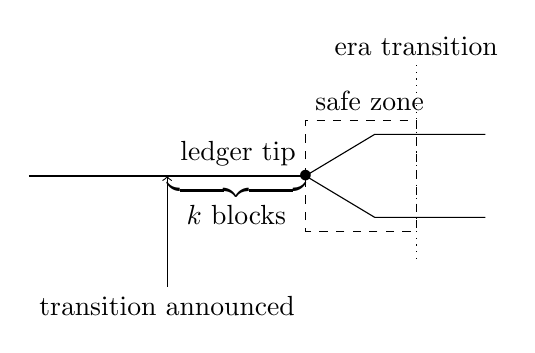
\begin{tikzpicture}[baseline=0pt]
\draw [thick] (-50pt,0) -- (50pt, 0) coordinate (tip);
\draw (tip) -- ++(25pt,  15pt) -- ++(40pt, 0pt);
\draw (tip) -- ++(25pt, -15pt) -- ++(40pt, 0pt);
\node at (tip) {$\bullet$};
\node at (tip) [above left] {ledger tip};
\draw [dashed] (tip)
            -- ++(0pt, 20pt) node[above right] {safe zone}
            -- ++(40pt, 0pt) coordinate (transition)
            -- ++(0pt, -40pt) -- ++(-40pt, 0pt) -- cycle;
\draw [dotted] (transition) ++(0pt, 20pt) node[above] {era transition}
            -- ++(0pt, -70pt);
\draw [<-] (tip) ++(-50pt, 0)
        -- +(0,-40pt) node[below] {transition announced};
% again, cheating...
\node at (25pt, -10pt) {$\underbrace{\hspace{50pt}}_\textrm{$k$ blocks}$};
\end{tikzpicture}
\end{equation}
%
How many slots are required to guarantee at least $k$ blocks is consensus
protocol specific; for example, for Praos this is typically set to $3k/f$ slots,
where $f$ is the active slot coefficient.

Many ledgers set the width of the safe zone such that it guarantees at least $k$
blocks, but \emph{in principle} there is no need for the width of the safe zone
to be related to $k$ at all, although other parts of consensus might have
requirements for the width of the safe zone; we will discuss that in the next
section (\cref{time:ledgerrestrictions:safezones}).

\subsection{Size of the safezones}
\label{time:ledgerrestrictions:safezones}

The most important example of where we might need to do time translation for
blocks ahead of the ledger's tip is forecasting the Shelley ledger view
(\cref{ledger:forecasting}). The Shelley ledger view contains an abstraction
called \lstinline!EpochInfo! allowing the ledger to do time conversions, for
example to decide when rewards should be allocated.

As discussed in \cref{forecast:ledgerview}, it is important that the forecast
range of the ledger to allow us to validate at least $k + 1$ blocks after the
ledger tip; consequently, the safe zone of the ledger must be wide enough to
guarantee that it can span $k + 1$ blocks. This combination of the requirements
of the ledger with the header/body split
(\cref{nonfunctional:network:headerbody}) means that in practice the width of
the safe zone should be at least equal to the forecast range of the ledger, and
hence defined in terms of $k$ after all.

\subsection{Stability should not be approximated}

We discussed in \cref{time:slots-vs-blocks} that the ledger uses uses slot
numbers to approximate stability. Such an approximation would violate
\cref{time-stable-under-evolution}, however. Although we never switch to a
shorter chain in terms of blocks, it is certainly possible that we might switch
to a chain with a smaller \emph{slot} number at its tip: this would happen
whenever we switch to a longer but denser chain. If stability would be based on
slot numbers, this might mean that we could go from a situation in which the era
transition is considered known (and hence the forecast extends into the next
era) to a situation in which the era transition is not yet considered known (and
hence the forecast range only includes the safe zone in the current era).

Admittedly such a reduction of the forecast range would be temporary, and once
the era transition is considered known again, it will be in the same location;
after all, the block that confirmed the era transition \emph{is} stable. This
means that any previously executed time conversions would remain to be valid;
however, the fact that the forecast range shrinks might lead to unexpected
surprises. The consensus layer therefore does not use the ledger's layer
notion of stability, but instead maintains additional state so that it can use
\emph{block} numbers rather than slot numbers to determine stability and be
able to determine stability precisely rather than approximate it.

\section{Properties}

\subsection{Forecast ranges arising from safe zones}

Slot length and epoch size can only change at era transitions. This means that
if the transition to the next era is not yet known, any time $t$ within the
era's safe zone is guaranteed to be within the era's forecast range. If the
transition to the next era \emph{is} known, the safe zone of the current era is
not relevant, but the safe zone of the next era is:
%
\begin{equation}
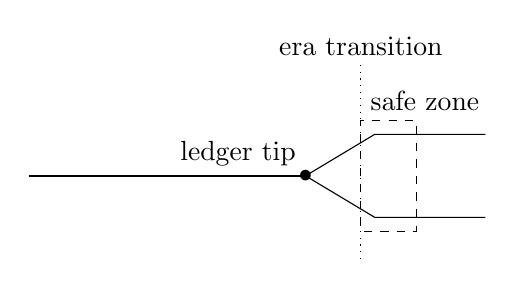
\begin{tikzpicture}[baseline=0pt]
\draw [thick] (-50pt,0) -- (50pt, 0) coordinate (tip);
\draw (tip) -- ++(25pt,  15pt) -- ++(40pt, 0pt);
\draw (tip) -- ++(25pt, -15pt) -- ++(40pt, 0pt);
\node at (tip) {$\bullet$};
\node at (tip) [above left] {ledger tip};
\draw [dashed] (tip) ++(20pt, 0pt) coordinate (transition)
            -- ++(0pt, 20pt) node[above right] {safe zone}
            -- ++(20pt, 0pt) -- ++(0pt, -40pt) -- ++(-20pt, 0pt) -- cycle;
\draw [dotted] (transition) ++(0pt, 40pt) node[above] {era transition}
            -- ++(0pt, -70pt);
\end{tikzpicture}
\end{equation}
%
The safe zone of the next era might be smaller or larger than (or indeed of
equal size as) the safe zone of the previous era; in this example it happens to
be smaller.

\Cref{hfc:era-transition-becoming-known} shows how the forecast range changes as
the next era transition becomes known; as shown, the next era starts at the
earliest possible moment (right after the safe zone); in general it could start
later than that, but of course not earlier (that would violate the definition of
the safe zone).

\begin{figure}

\begin{equation}
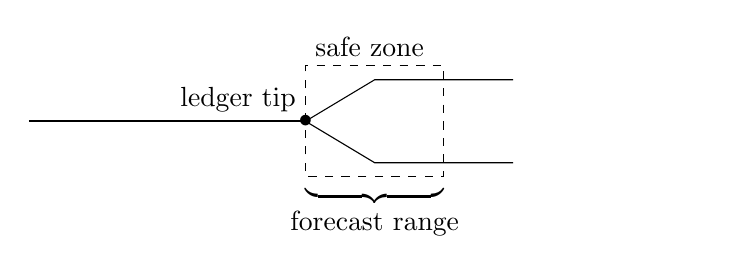
\begin{tikzpicture}[baseline=0pt]
\path (0,0) -- ++(200pt, 0pt); % adjust bounding box
\draw [thick] (-50pt,0) -- (50pt, 0) coordinate (tip);
\draw (tip) -- ++(25pt,  15pt) -- ++(50pt, 0pt);
\draw (tip) -- ++(25pt, -15pt) -- ++(50pt, 0pt);
\node at (tip) {$\bullet$};
\node at (tip) [above left] {ledger tip};
\draw [dashed] (tip)
            -- ++(0pt, 20pt) node[above right] {safe zone}
            -- ++(50pt, 0pt)
            -- ++(0pt, -40pt)
            -- ++(-50pt, 0pt) coordinate[pos=0.5] (safezone)
            -- cycle;
\node at (safezone) [below] {$\underbrace{\hspace{50pt}}_\textrm{forecast range}$};
\end{tikzpicture}
\end{equation}

\begin{equation}
\begin{tikzpicture}[baseline=0pt]
\path (0,0) -- ++(200pt, 0pt); % adjust bounding box
\draw [gray] (-50pt,0) -- (50pt, 0) coordinate (oldtip);
\draw [gray, name path=chaintop] (oldtip) -- ++(25pt, 15pt) coordinate[pos=0.25] (tip) -- ++(50pt, 0pt);
\draw [gray] (oldtip) -- ++(25pt, -15pt) -- ++(50pt, 0pt);
\draw [thick] (-50pt,0) -- (50pt, 0) -- (tip);
\node at (tip) {$\bullet$};
\node at (tip) [above left] {ledger tip};
\draw (tip) -- ++(25pt, 25pt) -- +(50pt, 0pt);
\draw (tip) -- ++(25pt, -5pt) -- +(50pt, 0pt);
\draw [dotted, name path=transition]
        (oldtip) ++(50pt, 60pt) node[above] {era transition}
              -- ++(0pt, -90pt);
\path [name intersections={of=transition and chaintop}]
        (intersection-1) coordinate (safezone);
\draw [dashed] (safezone)
            -- ++(0pt, 20pt) node[above right] {safe zone}
            -- ++(20pt, 0pt)
            -- ++(0pt, -40pt)
            -- ++(-20pt, 0pt) coordinate[pos=0.5] (safezone)
            -- cycle;

% cheat: we should compute this of course :)
\node at (90pt,-20pt) [below] {$\underbrace{\hspace{60pt}}_\textrm{forecast range}$};
\end{tikzpicture}
\label{forecast-range-known-era-transition}
\end{equation}
\caption{\label{hfc:era-transition-becoming-known}Era transition becoming known}
\end{figure}

\subsection{Cross-fork conversions}
\label{time:cross-fork}

\begin{lemma}[Cross fork conversions]
Suppose we have the ledger state at some point $P$, and want to do time
conversions for time $t$ of a point $Q$ on a different fork of the chain:

\begin{center}
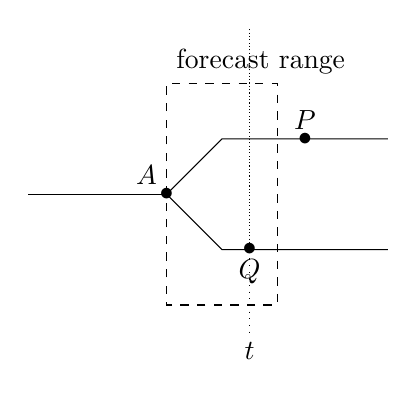
\begin{tikzpicture}
\draw (0,0) -- (50pt, 0) coordinate (A);
\draw (A) -- ++(20pt, 20pt)
          -- ++(30pt, 0) coordinate(P)
          -- ++(30pt, 0);
\draw (A) -- ++(20pt, -20pt)
          -- ++(10pt, 0) coordinate(Q1)
          -- ++(40pt, 0) coordinate(Q2)
          -- ++(10pt, 0);
\node at (A) {$\bullet$};
\node at (A) [above left] {$A$};
\node at (P) {$\bullet$};
\node at (P) [above] {$P$};
\node at (Q1) {$\bullet$};
\node at (Q1) [below] {$Q$};
\draw [dashed] (A) -- ++(0, 40pt) node[above right] {forecast range}
                   -- ++(40pt, 0)
                   -- ++(0, -80pt)
                   -- ++(-40pt, 0)
                   -- cycle;
\draw [dotted] (Q1) -- +(0, 80pt) -- +(0, -30pt) node[below] {$t$};
\end{tikzpicture}
\end{center}

Provided that $Q$ is within the forecast range of the common ancestor $A$
of $P$ and $Q$, the ledger state at $P$ can be used to do time conversions
for point $t$.
\end{lemma}

\begin{proof}
Since $t$ is within the forecast range at $A$, by definition $\timeconv{A}{t}$
is defined. By monotonicity (\cref{time-conversion-monotone}) we must have
\begin{align*}
\timeconv{A}{t} & = \timeconv{P}{t} \\
\timeconv{A}{t} & = \timeconv{Q}{t}
\end{align*}
It follows that $\timeconv{P}{t} = \timeconv{Q}{t}$.
\end{proof}

\section{Avoiding time}
\label{hfc:avoiding-time}

Time is complicated, and time conversions were pervasive throughout the
consensus layer. Despite the exposition above and the increased understanding,
we nonetheless have attempted to limit the use of time as much as possible,
in an attempt to simplify reasoning whenever possible. The use of
time within the core consensus layer is now very limited indeed:

\begin{enumerate}
\item When we check if we are a slot leader and need to produce a block, we
need to know the current time as a slot number (\todo{TODO.}We should discuss
this somewhere. The chapter on the consensus protocol discusses the protocol
side of things, but not the actual ``fork block production'' logic.)
\item When we add new blocks to the chain DB, we need to check if their slot
number is ahead of the wallclock (\cref{chainsel:infuture}).
\item Specific consensus protocols may need to do time conversions; for example,
Praos needs to know when various points in an epoch have been reached in order
to update nonces, switch stake distribution, etc.
\end{enumerate}

None of these use cases require either forecasting or cross-chain conversions.
The most important example of where forecasting is required is in projecting
the ledger view, as discussed in \cref{time:ledgerrestrictions:safezones}.
Cross-fork conversions (\cref{time:cross-fork}) may arise for example when the consensus layer makes time conversions available to tooling such as the wallet,
which may use it for example to show the wallclock of slots of blocks that may
not necessarily live on the current chain.

Keeping track of era transitions, and providing time conversions that take
them into account, is the responsibility of the hard fork combinator and
we will discuss it in more detail in \cref{hfc:time}.

In the remainder of this section we will discuss some simplifications
that reduced the reliance on time within the consensus layer.

\subsection{``Header in future'' check}
\label{time:header-infuture-check}

Recall from \cref{nonfunctional:network:headerbody} that block downloading
proceeds in two steps: first, the chain sync client downloads the block header
and validates it; if it finds that the header is valid, the block download logic
may decide to also download the block body, depending on chain selection
(\cref{consensus:overview:chainsel,consensus:class:chainsel}).

Suppose the node's own ledger state is at point $P$, and the incoming header is
at point $Q$. In order to validate the header, we need a ledger \emph{view} at
point $Q$ without having the ledger \emph{state} at point $Q$; this means that
point $Q$ must be within the ledger's forecast range at the common ancestor $A$
of $P$ and $Q$ (\cref{,ledger:forecasting}):

\begin{center}
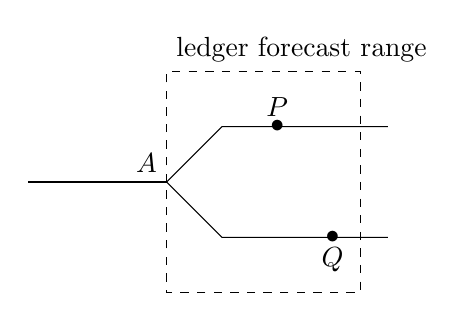
\begin{tikzpicture}
\draw (0, 0) -- (50pt, 0) coordinate (A);
\draw (A) -- ++(20pt,  20pt) -- ++(20pt, 0) coordinate (P) -- ++(40pt, 0);
\draw (A) -- ++(20pt, -20pt) -- ++(40pt, 0) coordinate (Q) -- ++(20pt, 0);
\node at (P) {$\bullet$};
\node at (Q) {$\bullet$};
\node at (A) [above left] {$A$};
\node at (P) [above] {$P$};
\node at (Q) [below] {$Q$};
\draw [dashed] (A) -- ++(0, 40pt) node[above right] {ledger forecast range}
                   -- ++(70pt, 0)
                   -- ++(0, -80pt)
                   -- ++(-70pt, 0)
                   -- cycle;
\end{tikzpicture}
\end{center}

As we have seen in \cref{time:cross-fork}, if $Q$ is within the \emph{time}
forecast range at $A$---put another way, if the time forecast range is at least
as wide as the ledger forecast range---then we also can use the ledger state at
$P$ to do time conversions at point $Q$. Moreover, as we saw in
\cref{time:ledgerrestrictions:safezones}, for many ledgers that inclusion
\emph{must} hold. If we make this a requirement for \emph{all} ledgers, in
principle the chain sync client could do a header-in-future check.

For simplicity, however, we nonetheless omit the check. As we will see in the
next section, the chain database must repeat this check \emph{anyway}, and so
doing it ahead of time in the chain sync client does not help very much;
skipping it avoids one more use of time within the consensus layer. Indeed, a
case could be made that we could skip header validation altogether, which would
alleviate the need for forecasting \emph{at all}; we will come back to this in
\cref{future:eliminating-forecasting}.

\subsection{Ahead-of-time ``block in future'' check}
\label{time:block-infuture-check}

In the original design of the chain database, when a new block was added we
first checked if the block's slot number was ahead of the wallclock, before
considering it for chain selection. If it was ahead of the wallclock by a small
amount (within the permissible clock skew), we then scheduled an action to
reconsider the block when its slot arrived.

In order to compare the block's slot number to the wallclock, we can either
convert the block's slot to a wallclock time, or convert the current wallclock
time to a slot number. Both are problematic: the only ledger state we have
available is our own current ledger state, which may not be usable to translate
the current wallclock time to a slot number, and since we don't know anything
about the provenance of the block (where the block came from), that ledger state
may also not be usable to translate the block's slot number to a wallclock
time. We now circumvent this problem by delaying the in-future check until we
have validated the block, and so can use the block's \emph{own} ledger state to
do the time conversion (\cref{chainsel:infuture}).

We saw in the previous section that the chain sync client \emph{could} do the
in-future check on headers, but the chain sync client is not the only way that
blocks can be added to the chain database, so simply skipping the check in the
chain database altogether, stipulating as a \emph{precondition} that the block
is not ahead of the wallclock, is not a good idea. Nonetheless it is worth
considering if we could use a weaker precondition, merely requiring that the
node's current ledger tip must be usable for time conversions for the slot
number of the new block. Specifically, can we guarantee that we can satisfy this
precondition in the chain sync client, if we do the in-future check on headers
after all?

It turns out that in general we cannot, not even in relatively common cases.
Consider again the diagram from \cref{time:header-infuture-check}, but
specialised to the typical case that the upstream node is on the same chain as
we are, but a bit ahead of us:

\begin{center}
\begin{tikzpicture}
\path (0,0) -- ++(200pt, 0pt); % adjust bounding box
\draw (0, 0) -- (50pt, 0) coordinate (A) coordinate (P);
\draw (A) -- ++(20pt, 0pt) -- ++(20pt, 0) -- ++(40pt, 0);
\draw (A) -- ++(20pt, 0pt) -- ++(40pt, 0) coordinate (Q) -- ++(20pt, 0);
\node at (P) {$\bullet$};
\node at (Q) {$\bullet$};
\node at (A) [above left] {$A$};
\node at (A) {$\bullet$};
\node at (P) [below left] {$P$};
\node at (Q) [below] {$Q$};
\draw [dashed] (A) -- ++(0, 20pt) node[above right] {forecast range}
                   -- ++(70pt, 0)
                   -- ++(0, -40pt)
                   -- ++(-70pt, 0)
                   -- cycle;
\end{tikzpicture}
\end{center}

Since $P$ and $Q$ are on the same chain,  point $P$ is necessarily also the
``intersection'' point, and the distance between $P$ and $Q$ can only arise from
the block download logic lagging behind the chain sync client.
Now consider what happens when the node switches to an alternative fork:

\begin{center}
\begin{tikzpicture}
\path (0,0) -- ++(200pt, 0pt); % adjust bounding box
\draw (0, 0) -- (30pt, 0) coordinate (A);
\draw (A) -- ++(20pt,  20pt) -- ++(20pt, 0) coordinate (P) -- ++(60pt, 0);
\draw (A) -- ++(20pt, -20pt) -- ++(60pt, 0) coordinate (Q) -- ++(20pt, 0);
\node at (P) {$\bullet$};
\node at (Q) {$\bullet$};
\node at (A) [above left] {$A$};
\node at (P) [above] {$P$};
\node at (Q) [below] {$Q$};
\draw [dashed] (A) -- ++(0, 40pt) node[above right] {forecast range}
                   -- ++(70pt, 0)
                   -- ++(0, -80pt)
                   -- ++(-70pt, 0)
                   -- cycle;
\end{tikzpicture}
\end{center}

Note what happens: since the node is switching to another fork, it must rollback
some blocks and then roll forward; consequently, the intersection point $A$
moves back, and $P$ moves forward (albeit on a different chain). $Q$ stays the
same, \emph{but might have fallen out of the forecast range at $A$}.

This means that even if the chain sync client was able to verify that a header
(at point $Q$) was not ahead of the wallclock, if the node switches to a
different fork before the block download logic has downloaded the corresponding
block, when it presents that downloaded block to the chain database, the block
might no longer be within the forecast range of the node's current ledger and
the chain database will not be able to verify (ahead of time) whether or not the
block is ahead of the wallclock. What's worse, unlike the chain sync client, the
chain database has no access to the intersection point $A$; it all it has is the
ledger's current tip at  point $P$ and the new block at point $Q$. It therefore
has no reliable way of even determining \emph{if} it can do time conversions for
the new block.

\subsection{``Immutable tip in future'' check}
\label{time:imm-tip-in-future}

The chain database never adopts blocks from the future
(\cref{chainsel:infuture}). Nevertheless, it is possible that if the user sets
their computer system clock back by (the equivalent of) more than $k$ blocks,
the immutable database (\cref{storage:components}) might contain blocks
whose slot numbers are ahead of the wall clock. We cannot verify this during a
regular integrity check of the immutable database because, as we have seen in
this chapter, we would need a ledger state to do so, which we are not
constructing during that integrity check. For now, we simply omit this check
altogether, declaring it to be the user's responsibility instead to do a
fresh install if they do reset their clock by this much.

However, in principle this check is not difficult: we initialise the immutable
DB \emph{without} doing the check, then initialise the ledger DB, passing it the
immutable DB (which it needs to replay the most recent blocks, see
\cref{ledgerdb}), and then ask the ledger DB for the ledger state
corresponding to the tip of the immutable database. That ledger state will then
allow us to do time conversions for any of the blocks in the immutable DB,
trimming any blocks that are ahead of the wallclock.

\subsection{Scheduling actions for slot changes}
\label{time:scheduling-actions}

The consensus layer provides an abstraction called \lstinline!BlockchainTime!
that provides access to the current slot number. It also offers an interface
for scheduling actions to be run on every slot change. However, if the node
is still syncing with the chain, and does not have a recent ledger state
available, the current slot number, and indeed the current slot length,
are simply unknown. In this case the blockchain time will report the current
slot number as unavailable, and any scheduled actions will not be run.

We therefore limit the use of this scheduler to a single application only:
it is used to trigger the leadership check (and corresponding block
production, if we find we are a leader). This means that the leadership
check will not be run if we are still syncing with the chain and have no
recent ledger state available, but that is correct: producing blocks based on
ancient ledger states is anyway not useful.

\subsection{Switching on ``deadline mode'' in the network layer}

Under normal circumstances, the priority of the network layer is to reduce
\emph{latency}: when a block is produced, it must be distributed across the
network as soon as possible, so that the next slot leader can construct the
\emph{next} block as this block's successor; if the block arrives too late,
the next slot leader will construct their block as the successor of the previous
block instead, and the chain temporarily forks.

When we are far behind, however, the priority is not to reduce latency, but
rather to improve \emph{throughput}: we want to catch up as quickly as we can
with the chain, and aren't producing blocks anyway
(\cref{time:scheduling-actions}).

In order to switch between these two modes we want to know if we are near the
tip of the ledger---but how can we tell? If we know the current slot number
(the slot number corresponding to the current wall clock), we can compare
that current slot number to the slot number at the tip of the ledger. But,
as we mentioned before, if we are far behind, the current slot number of
simply unknown. Fortunately, we can use this to our advantage: if the
slot number is unknown, we \emph{must} be far behind, and hence we can use
the decision, turning on deadline mode only if the slot number is known
\emph{and} within a certain distance from the ledger tip.
